% This is the Reed College LaTeX thesis template. Most of the work
% for the document class was done by Sam Noble (SN), as well as this
% template. Later comments etc. by Ben Salzberg (BTS). Additional
% restructuring and APA support by Jess Youngberg (JY).
% Your comments and suggestions are more than welcome; please email
% them to cus@reed.edu
%
% See http://web.reed.edu/cis/help/latex.html for help. There are a
% great bunch of help pages there, with notes on
% getting started, bibtex, etc. Go there and read it if you're not
% already familiar with LaTeX.
%
% Any line that starts with a percent symbol is a comment.
% They won't show up in the document, and are useful for notes
% to yourself and explaining commands.
% Commenting also removes a line from the document;
% very handy for troubleshooting problems. -BTS

% As far as I know, this follows the requirements laid out in
% the 2002-2003 Senior Handbook. Ask a librarian to check the
% document before binding. -SN

%%
%% Preamble
%%
% \documentclass{<something>} must begin each LaTeX document
\documentclass[12pt,twoside]{reedthesis}
% Packages are extensions to the basic LaTeX functions. Whatever you
% want to typeset, there is probably a package out there for it.
% Chemistry (chemtex), screenplays, you name it.
% Check out CTAN to see: http://www.ctan.org/
%%
\usepackage{graphicx,latexsym}
\usepackage{amsmath}
\usepackage{amssymb,amsthm}
\usepackage{longtable,booktabs,setspace}
\usepackage{chemarr} %% Useful for one reaction arrow, useless if you're not a chem major
\usepackage[hyphens]{url}
% Added by CII
\usepackage{hyperref}
\usepackage{lmodern}
\usepackage{float}
\floatplacement{figure}{H}
% End of CII addition
\usepackage{rotating}

% Next line commented out by CII
%%% \usepackage{natbib}
% Comment out the natbib line above and uncomment the following two lines to use the new
% biblatex-chicago style, for Chicago A. Also make some changes at the end where the
% bibliography is included.
%\usepackage{biblatex-chicago}
%\bibliography{thesis}


% Added by CII (Thanks, Hadley!)
% Use ref for internal links
\renewcommand{\hyperref}[2][???]{\autoref{#1}}
\def\chapterautorefname{Chapter}
\def\sectionautorefname{Section}
\def\subsectionautorefname{Subsection}
% End of CII addition

% Added by CII
\usepackage{caption}
\captionsetup{width=5in}
% End of CII addition

% \usepackage{times} % other fonts are available like times, bookman, charter, palatino

% Syntax highlighting #22
  \usepackage{color}
  \usepackage{fancyvrb}
  \newcommand{\VerbBar}{|}
  \newcommand{\VERB}{\Verb[commandchars=\\\{\}]}
  \DefineVerbatimEnvironment{Highlighting}{Verbatim}{commandchars=\\\{\}}
  % Add ',fontsize=\small' for more characters per line
  \usepackage{framed}
  \definecolor{shadecolor}{RGB}{248,248,248}
  \newenvironment{Shaded}{\begin{snugshade}}{\end{snugshade}}
  \newcommand{\KeywordTok}[1]{\textcolor[rgb]{0.13,0.29,0.53}{\textbf{#1}}}
  \newcommand{\DataTypeTok}[1]{\textcolor[rgb]{0.13,0.29,0.53}{#1}}
  \newcommand{\DecValTok}[1]{\textcolor[rgb]{0.00,0.00,0.81}{#1}}
  \newcommand{\BaseNTok}[1]{\textcolor[rgb]{0.00,0.00,0.81}{#1}}
  \newcommand{\FloatTok}[1]{\textcolor[rgb]{0.00,0.00,0.81}{#1}}
  \newcommand{\ConstantTok}[1]{\textcolor[rgb]{0.00,0.00,0.00}{#1}}
  \newcommand{\CharTok}[1]{\textcolor[rgb]{0.31,0.60,0.02}{#1}}
  \newcommand{\SpecialCharTok}[1]{\textcolor[rgb]{0.00,0.00,0.00}{#1}}
  \newcommand{\StringTok}[1]{\textcolor[rgb]{0.31,0.60,0.02}{#1}}
  \newcommand{\VerbatimStringTok}[1]{\textcolor[rgb]{0.31,0.60,0.02}{#1}}
  \newcommand{\SpecialStringTok}[1]{\textcolor[rgb]{0.31,0.60,0.02}{#1}}
  \newcommand{\ImportTok}[1]{#1}
  \newcommand{\CommentTok}[1]{\textcolor[rgb]{0.56,0.35,0.01}{\textit{#1}}}
  \newcommand{\DocumentationTok}[1]{\textcolor[rgb]{0.56,0.35,0.01}{\textbf{\textit{#1}}}}
  \newcommand{\AnnotationTok}[1]{\textcolor[rgb]{0.56,0.35,0.01}{\textbf{\textit{#1}}}}
  \newcommand{\CommentVarTok}[1]{\textcolor[rgb]{0.56,0.35,0.01}{\textbf{\textit{#1}}}}
  \newcommand{\OtherTok}[1]{\textcolor[rgb]{0.56,0.35,0.01}{#1}}
  \newcommand{\FunctionTok}[1]{\textcolor[rgb]{0.00,0.00,0.00}{#1}}
  \newcommand{\VariableTok}[1]{\textcolor[rgb]{0.00,0.00,0.00}{#1}}
  \newcommand{\ControlFlowTok}[1]{\textcolor[rgb]{0.13,0.29,0.53}{\textbf{#1}}}
  \newcommand{\OperatorTok}[1]{\textcolor[rgb]{0.81,0.36,0.00}{\textbf{#1}}}
  \newcommand{\BuiltInTok}[1]{#1}
  \newcommand{\ExtensionTok}[1]{#1}
  \newcommand{\PreprocessorTok}[1]{\textcolor[rgb]{0.56,0.35,0.01}{\textit{#1}}}
  \newcommand{\AttributeTok}[1]{\textcolor[rgb]{0.77,0.63,0.00}{#1}}
  \newcommand{\RegionMarkerTok}[1]{#1}
  \newcommand{\InformationTok}[1]{\textcolor[rgb]{0.56,0.35,0.01}{\textbf{\textit{#1}}}}
  \newcommand{\WarningTok}[1]{\textcolor[rgb]{0.56,0.35,0.01}{\textbf{\textit{#1}}}}
  \newcommand{\AlertTok}[1]{\textcolor[rgb]{0.94,0.16,0.16}{#1}}
  \newcommand{\ErrorTok}[1]{\textcolor[rgb]{0.64,0.00,0.00}{\textbf{#1}}}
  \newcommand{\NormalTok}[1]{#1}

% To pass between YAML and LaTeX the dollar signs are added by CII
\title{Ballot Completion in Ranked Choice Voting}
\author{Jay Lee}
% The month and year that you submit your FINAL draft TO THE LIBRARY (May or December)
\date{May 2019}
\division{Mathematics and Natural Sciences}
\advisor{Heather Kitada Smalley}
\institution{Reed College}
\degree{Bachelor of Arts}
%If you have two advisors for some reason, you can use the following
% Uncommented out by CII
% End of CII addition

%%% Remember to use the correct department!
\department{Mathematics - Statistics}
% if you're writing a thesis in an interdisciplinary major,
% uncomment the line below and change the text as appropriate.
% check the Senior Handbook if unsure.
%\thedivisionof{The Established Interdisciplinary Committee for}
% if you want the approval page to say "Approved for the Committee",
% uncomment the next line
%\approvedforthe{Committee}

% Added by CII
%%% Copied from knitr
%% maxwidth is the original width if it's less than linewidth
%% otherwise use linewidth (to make sure the graphics do not exceed the margin)
\makeatletter
\def\maxwidth{ %
  \ifdim\Gin@nat@width>\linewidth
    \linewidth
  \else
    \Gin@nat@width
  \fi
}
\makeatother

\renewcommand{\contentsname}{Table of Contents}
% End of CII addition

\setlength{\parskip}{0pt}

% Added by CII

\providecommand{\tightlist}{%
  \setlength{\itemsep}{0pt}\setlength{\parskip}{0pt}}

\Acknowledgements{
I want to thank a few people.
}

\Dedication{
You can have a dedication here if you wish.
}

\Preface{
This is an example of a thesis setup to use the reed thesis document
class (for LaTeX) and the R bookdown package, in general.
}

\Abstract{
One of the arguments against implementing ranked-choice voting (RCV) is
that RCV is harder for voters to participate in. Two of the reasons for
this are the more complicated ballot design and the extra effort that
goes into forming a ordered preference of candidates. To evaluate this
claim, we examine rates of ballot errors and undervoting (ranking fewer
than the allowed number of candidates) in some American elections
conducted with RCV. Results show that idk yet. \par

Second paragraph of abstract starts here.
}

% End of CII addition
%%
%% End Preamble
%%
%

\usepackage{amsthm}
\newtheorem{theorem}{Theorem}[chapter]
\newtheorem{lemma}{Lemma}[chapter]
\theoremstyle{definition}
\newtheorem{definition}{Definition}[chapter]
\newtheorem{corollary}{Corollary}[chapter]
\newtheorem{proposition}{Proposition}[chapter]
\theoremstyle{definition}
\newtheorem{example}{Example}[chapter]
\theoremstyle{definition}
\newtheorem{exercise}{Exercise}[chapter]
\theoremstyle{remark}
\newtheorem*{remark}{Remark}
\newtheorem*{solution}{Solution}
\begin{document}

% Everything below added by CII
  \maketitle

\frontmatter % this stuff will be roman-numbered
\pagestyle{empty} % this removes page numbers from the frontmatter
  \begin{acknowledgements}
    I want to thank a few people.
  \end{acknowledgements}
  \begin{preface}
    This is an example of a thesis setup to use the reed thesis document
    class (for LaTeX) and the R bookdown package, in general.
  \end{preface}
  \hypersetup{linkcolor=black}
  \setcounter{tocdepth}{2}
  \tableofcontents

  \listoftables

  \listoffigures
  \begin{abstract}
    One of the arguments against implementing ranked-choice voting (RCV) is
    that RCV is harder for voters to participate in. Two of the reasons for
    this are the more complicated ballot design and the extra effort that
    goes into forming a ordered preference of candidates. To evaluate this
    claim, we examine rates of ballot errors and undervoting (ranking fewer
    than the allowed number of candidates) in some American elections
    conducted with RCV. Results show that idk yet. \par
    
    Second paragraph of abstract starts here.
  \end{abstract}
  \begin{dedication}
    You can have a dedication here if you wish.
  \end{dedication}
\mainmatter % here the regular arabic numbering starts
\pagestyle{fancyplain} % turns page numbering back on

\chapter*{Introduction}\label{introduction}
\addcontentsline{toc}{chapter}{Introduction}

Welcome to the \emph{R Markdown} thesis template. This template is based
on (and in many places copied directly from) the Reed College LaTeX
template, but hopefully it will provide a nicer interface for those that
have never used TeX or LaTeX before. Using \emph{R Markdown} will also
allow you to easily keep track of your analyses in \textbf{R} chunks of
code, with the resulting plots and output included as well. The hope is
this \emph{R Markdown} template gets you in the habit of doing
reproducible research, which benefits you long-term as a researcher, but
also will greatly help anyone that is trying to reproduce or build onto
your results down the road.

Hopefully, you won't have much of a learning period to go through and
you will reap the benefits of a nicely formatted thesis. The use of
LaTeX in combination with \emph{Markdown} is more consistent than the
output of a word processor, much less prone to corruption or crashing,
and the resulting file is smaller than a Word file. While you may have
never had problems using Word in the past, your thesis is likely going
to be about twice as large and complex as anything you've written
before, taxing Word's capabilities. After working with \emph{Markdown}
and \textbf{R} together for a few weeks, we are confident this will be
your reporting style of choice going forward.

\textbf{Why use it?}

\emph{R Markdown} creates a simple and straightforward way to interface
with the beauty of LaTeX. Packages have been written in \textbf{R} to
work directly with LaTeX to produce nicely formatting tables and
paragraphs. In addition to creating a user friendly interface to LaTeX,
\emph{R Markdown} also allows you to read in your data, to analyze it
and to visualize it using \textbf{R} functions, and also to provide the
documentation and commentary on the results of your project. Further, it
allows for \textbf{R} results to be passed inline to the commentary of
your results. You'll see more on this later.

\textbf{Who should use it?}

Anyone who needs to use data analysis, math, tables, a lot of figures,
complex cross-references, or who just cares about the final appearance
of their document should use \emph{R Markdown}. Of particular use should
be anyone in the sciences, but the user-friendly nature of
\emph{Markdown} and its ability to keep track of and easily include
figures, automatically generate a table of contents, index, references,
table of figures, etc. should make it of great benefit to nearly anyone
writing a thesis project.

\chapter{What is ranked choice voting?}\label{litreview}

Ranked choice voting (RCV), also known as the alternative vote (AV) or
instant-runoff voting (IRV) is an alternative voting method to the
first-past-the-post (FPTP) or ``plurality'' election system more
familiar to American voters, where the candidate with the most votes
wins. Each voter, instead of choosing their highest preference among a
set of candidates for an office, ranks some subset of the candidates in
order of preference. This system (or a close variant) is used in
Australia, Maine, and some American municipalities: San Francisco, CA;
Minneapolis, MN; and Cambridge, MA; among others.

The single-winner RCV tabulation algorithm generally proceeds as
follows:
\begin{enumerate}
\def\labelenumi{\arabic{enumi}.}
\item
  For each voter, identify their most preferred candidate that has not
  yet been eliminated. Count up these preferences by candidate.
\item
  If one candidate has a majority (50\% + 1) of the unexhausted votes,
  they are declared the winner and counting stops.
\item
  The candidate with the lowest number of votes is eliminated.
\item
  The ballots counted for that candidate are each transferred to the
  voter's next choice if one exists, or if one does not exist the ballot
  is ``exhausted'' and removed from counting for further rounds.
\item
  Return to 1.
\end{enumerate}
Most jurisdictions that use RCV have slightly different rules for edge
cases and ballot errors, but this algorithm is what distinguishes RCV
from other ranked voting systems (e.g.
\href{https://www.electoral-reform.org.uk/voting-systems/types-of-voting-system/borda-count/}{Borda},
\href{http://web.math.princeton.edu/math_alive/Voting/Lab1/Condorcet.html}{Condorcet},
\href{https://www.uk-engage.org/2013/09/electoral-systems-whats-the-difference-between-contingent-voting-and-alternative-voting-systems/}{Contingent},
etc.). A close variant of RCV is the single transferrable vote (STV)
method\footnote{More accurately, RCV is the single-winner implementation
  of the STV algorithm.}, which can be used to elect multiple
candidates, i.e.~for a school board, instead of just one. In the US,
this is used in Cambridge, MA and Minneapolis, MN to elect multi-member
offices.

\section{Frequently Used Terms}\label{frequently-used-terms}

Below are some definitions for frequently used terms later on. These are
not all ubiquitous (for example, ``undervote'' has another meaning in
most voting research), but we define them here for clarity later on.
\begin{itemize}
\item
  \emph{Overvote}: when a voter ranks multiple candidates in the same
  slot. This slot is typically thrown out entirely in counting, because
  it's often not possible to determine which candidate was preferred.
\item
  \emph{Undervote}: when a voter does not rank candidates in all of the
  slots available to them. This is different than other definitions of
  ``undervote'', which refer to a voter participating in one election on
  a ballot but not another one. This is not a problem in counting, and
  is explicitly allowed in the laws of most jurisdictions. A plurality
  election analog would be voting in high-profile races
  (e.g.~presidential), but not down-ticket decisions (e.g.~local water
  board).
\item
  \emph{Skipped vote}: when a voter ranks no candidate at slot \(x\),
  but ranks a candidate at slot \(y > x\). This is typically not a
  problem in counting, but different jurisdictions have different rules
  about whether a voter's ballot is exhausted at this point or continues
  on to their next ranked choice. Plurality voting has no analog to
  this, because each race only has one ``ranking'' (first!).
\item
  \emph{Duplicated vote}: when a voter ranks the same candidate for
  distinct slots \(x\) and \(y\). This is typically not a problem for
  counting, and the first ranking for the candidate is used. Similar to
  a skipped vote, plurality voting has no analog to this.
\item
  \emph{Ballot exhaustion}: as ballot counting progresses, some ballots
  will become ``exhausted'' when all the candidates selected are
  eliminated. Suppose the final count in an election is between
  candidates B and D, and a voter ranked candidates C-A-E. Their ballot
  would not be counted in this final round, as they expressed no
  preference for either candidate B or D. An analogous situation in a
  plurality election might be voting in the general election but not a
  runoff, that is only having a say in part of the election.
\end{itemize}
Over-, skipped, and duplicated votes are really only interpretable as
``ballot mistakes'': for example, even if a voter truly prefers two
candidates equally, the ballot instructions (should) make it clear that
ranking them at the same slot is not allowed.

\section{Claims about RCV}\label{claims-about-rcv}

There are plenty of arguments both for and against implementing RCV in
place of plurality in different jurisdictions (see the literature
review), but here we'll focus on evaluating one major argument against
it - RCV is harder for voters to participate in than a plurality system.
There are two major reasons cited for this:
\begin{itemize}
\item
  The physical design of an RCV ballot is usually more complicated than
  a plurality ballot, because there has to be a system to encode a more
  full preference among the candidates than just selecting one candidate
\item
  The process of forming a multi-candidate preference inherently takes
  more mental energy than just choosing a favorite candidate
\end{itemize}
The first facet of this argument should be reflected in ballot errors
made by voters. Compared to plurality voting, we expect more errors in
an RCV ballot just because the ballot is more complicated. There are
also more potentials for error in the RCV system generally. The only
``errors'' in a plurality ballot are incompletely marking a candidate
(think incorrect Scantron bubbling, or hanging chads) or overvoting,
both of which are potential pitfalls for a ranked choice ballot as well.
On top of these, there are the potential errors of duplicated and
skipped votes unique to ranked ballots\footnote{These types of errors
  are not uniform, and some jurisdictions are more forgiving than others
  about rules for counting these errors. While it may be apparent that a
  voter who listed the same candidate 3 times (A-A-A) prefers that
  candidate, a candidate ranking of A-B-A is harder to extract a clear
  preference from. Skipped votes are where we see the most variance in
  jurisdiction counting rules: if a voter marks the ballot A-\_\_-B,
  skipping the second slot, some jurisdictions will ignore the skip and
  treat B as the voter's second choice, while others will stop counting
  after A is eliminated (ignoring their vote for B), and others yet will
  throw out the ballot entirely.}.

The second facet should be reflected in incomplete ballots filled out by
voters. Given that they understand how to encode their preferences on
the ballot, there is still the non-trivial task of forming such a
preference. Structurally, some of the factors that should affect this
incompleteness are:
\begin{itemize}
\item
  The number of candidates running for a position
\item
  The number of candidates voters can rank
\item
  The number of seats elected in a given race
\end{itemize}
This first variable is at the election level (different for every
election), the second is at the jurisdiction level, and the third is a
mix of both. For a clear example of these differences, consider a
\href{https://sfelections.org/results/20161108/data/20161206/d3/20161206_d3.pdf}{2016
San Francisco Board of Supervisors race (District 3)} versus a
\href{https://www.cambridgema.gov/election2017/Council\%20Order\%20Round.htm}{2017
Cambridge City Council race}.
\begin{longtable}[]{@{}lll@{}}
\toprule
Factor & San Francisco 2016 & Cambridge 2017\tabularnewline
\midrule
\endhead
Candidates running & 2 & 27\tabularnewline
Candidates rankable & 2 (Generally, up to 3\footnote{This is changing in
  2019 to be up to 10.}) & 27 (Generally, all)\tabularnewline
Seats elected & 1 & 9\tabularnewline
\bottomrule
\end{longtable}
\section{History of RCV in the US (SF in
particular)}\label{history-of-rcv-in-the-us-sf-in-particular}

In the United States, there have been two major periods of RCV
implementation in various jurisdictions. Between 1915 and 1950, 24
American cities chose to institute RCV as a form of local election. By
1965, however, all of these except for Cambridge, MA had eliminated the
policy change. Then, in the 2000s, there was a resurgence of uptake in a
different set of American cities\footnote{Mostly in the American West:
  there are 9 cities west of the Mississippi River
  \href{https://www.fairvote.org/where_is_ranked_choice_voting_used}{currently
  using RCV} and only 4 east of it}, including Minneapolis and a handful
in the San Francisco Bay Area. While Cambridge has consistently used the
multi-winner (STV) method to elect City Council and School Board seats,
the modern resurgence of RCV almost universally deals with single-winner
elections. Research argues that RCV appears in jurisdictions where there
is strong multi-party support for the reform - the RCV method itself
gives individual parties less power in the election process, so powerful
single parties usually don't have reason to support it.

\section{Why, or why not, implement
RCV?}\label{why-or-why-not-implement-rcv}

There are plenty of arguments on both sides of implementing RCV in
jurisdictions that consider it.

\subsection{Pros}\label{pros}

\subsubsection{No secondary elections}\label{no-secondary-elections}

There are two major types of ``secondary elections'' used in American
voting: primary elections and runoff elections. Primaries are used by
political parties to select their nominee for a general election, so the
voters of any one party aren't split between different candidates.
Runoffs are most often used when no candidate in the general election
surpasses 50\% of the vote total. Typically the top two candidates from
the general election\footnote{Or primary election - Seven Southern
  states require primary winners to obtain 50\% of the vote to get on
  the general election ballot, and some other states have a requirement
  of 40\%. (WaPo article)} advance to a later runoff. These secondary
elections face two main challenges: low turnout and high cost.

Secondary elections as a whole face low turnout (Wright, 1989; Ranney,
1972). Reasons: Research shows that people don't actually like voting
that much - the more frequently elections are held, the lower turnout
will be for all of them generally (Boyd, 1986). Secondary elections
increase the number of elections in a period, so this is one possible
reason why they generally have low turnout. Further research indicates
that holding elections concurrently with a presidential election
``increase{[}s{]} the likelihood that citizens will vote'' (Boyd, 1986).
This is seen in off-year Congressinoal elections, where turnout drops
from presidential years. Typically general elections are held
concurrently with presidential elections (second Tuesday in November,
super high media coverage, lots of voter outreach, yadda yadda), so
secondary elections cannot be held at the same time as a presidential
election and they should thus suffer in turnout. This low turnout has
consequences for representation in the system. The same research
(Ranney, 1972) finds that while primary voters are not ideologically
unrepresentative of general election voters, they are both
demographically unrepresentative and unrepresentative on some major
issues. Traditional knowledge holds that primary voters are more
committed partisans than general election voters, leading the eventual
candidates in a general election to be polarized away from the
``center'' of political ideas (double check this but I'm pretty sure the
cite is Hill's \emph{Instant Runoff Voting}).

The higher costs associated with secondary elections are a little more
intuitive than turnout issues - it takes money to hold elections.
Pollworkers have to be paid, facilities have to be reserved, and
candidates have to do more campaigning. A 2011 City Council runoff in
Plano, TX cost the city an extra \$73,000 (Plano Star Courier, 2011). A
2012 Alabama runoff for multiple seats cost the state about \$3 million.

Since RCV eliminates the need for primary and runoff elections while
still ensuring majority rule (which is the main reason for these
elections), it should avoid the problems of lower turnout and higher
costs associated with secondary elections\footnote{Or at least some of
  it - costs overall are indeterminate (Rhode comference paper)}. Summed
up, RCV decreases costs and ``boosts turnout via elimination of
low-turnout elections'' (Morales, 2018).

\subsubsection{Ensures majority rule}\label{ensures-majority-rule}

In jurisdictions without rules for 50\% minimums, a common phenomenon is
a candidate winning an election with less than 50\% of the vote (a
plurality, rather than a majority). The major conceptual issue with this
is that more people preferred a candidate other than the one who was
elected\footnote{The `ideal' for electoral systems is the Condorcet
  condition: the candidate elected should beat all other candidates in
  one-on-one contests.}. RCV requires that a winning candidate receive
at least 50\% of the votes remaining\footnote{See below for issues with
  this `remaining' concept.}, ensuring that a majority of voters prefer
the elected candidate to other candidates.

This is particularly important in jurisdictions (like Maine) with strong
third-party support and more than two viable candidates. Former Maine
Governor Paul LePage, a Republican, won his first election in 2010 with
38.1\% of the vote, compared to Independent Eliot Cutler's
36.7\%\footnote{a margin of about 7,500 votes. Democrat Libby Mitchell
  received 19\%.}.

\subsubsection{Reduces strategic voting - spoiler candidates and third
parties}\label{reduces-strategic-voting---spoiler-candidates-and-third-parties}

Strategic voting\footnote{Also known as ``tactical'' or ``insincere''
  voting.} is a scenario where a voter does not reflect their true
preferences on their cast ballot in order to affect the outcome of the
election. For example, a third party supporter may cast their vote for
one of the two major party candidates because otherwise they feel like
``it won't count''.

The ``spoiler effect'' is when a third party candidate draws votes away
from the ideologically closest major party candidate, thus contributing
to the election of the other major party candidate. The most recent
large-scale accusation of this was in the 2000 election. Green Party
candidate Ralph Nader drew about 3\% of the national vote, more than the
margin of victory for George W. Bush over Al Gore\footnote{Admittedly,
  the margins are less clear-cut than this at the state level, where the
  margins actually matter for the Electoral College.}. In the especially
consequential state of Florida, Nader took 1.6\% of the vote: almost 200
times greater than the margin between the two major party candidates of
less than .01 percentage points\footnote{Not to point fingers at Nader
  alone in this case - while he was the most popular third party
  candidate by far, all 8 official third-party candidates received more
  votes than the major-candidate margin of only 537 votes} (source from
FEC). Many believed that Nader, generally seen as more liberal than the
Democrat Gore, drew votes from the Democratic base that would have
helped Gore win the election otherwise. While research into third-party
voters casts some doubt on this theory's applicability in 2000 (Herron,
Lewis)\footnote{In short - while Nader's Florida voters potentially
  would have broken enough for Gore to put him over the top, this was
  more a factor of the unusually close margin between the two major
  candidates than anything that Nader aided in particular.}, public
opinion still rests on the idea that Nader cost Gore the
presidency\footnote{One of the sections of Nader's Wikipedia page is
  entitled ``Spoiler controversy'' in regards to this election.}. In
fact, a pro-Republican PAC aired campaign ads promoting Nader in
Democratic states in an attempt to pull votes from Gore (Meckler, 2000).

One of the reasons for major party voters to support RCV is that is
avoids this spoiler issue. Under a plurality system, voters are
discouraged from voting for third-party candidates because it could help
elect their least-preferred of the two major candidates - ``the greater
of two evils'', so to speak. Under RCV, however, since voters can be
heard throughout multiple rounds across separate candidates, third-party
voters can vote for their most preferred candidate, then still have
their vote count for a better major-party candidate if their first
option is eliminated.

Conversely, one of the reasons for third-party voters to support RCV is
that it helps third party candidates get elected. Voters can ignore this
aforementioned facet of strategic voting\footnote{Or any strategic
  voting - while not impossible, it's infeasible to vote strategically
  under RCV (Bartholdi and Orlin, 1990).} and select their truly
preferred candidate. Third-party supporters who were worried about the
spoiler effect, then, can vote for their true preference of a third
party and not inadvertently help a less-preferred major candidate get
elected. As people abandon this strategy, third parties will receive
more votes from people no longer worried about the spoiler effect, and
this could get third party candidates elected.

\subsubsection{Disincentivizes negative
campaigning}\label{disincentivizes-negative-campaigning}

Ranked choice voting should incentivize candidates to avoid negative
campaigning. In a plurality election, since candidates don't care about
voters who are committed to their competitors, a well-thought out
negative campaign will only ostracize voters who were never going to
support another candidate in the first place, and perhaps bring more
swing voters to their side. Under RCV, however, alienating another
candidate's voters could backfire in the event that candidate is
eliminated and these voters decide to support your opponent in the next
round, causing your defeat . Research supports this - a 2016 study
showed that voters in cities using RCV are more satisfied with campaigns
than in cities who use plurality methods, and consider the campaign to
have a less negative tone overall (Donovan et al.). In San Francisco's
first RCV election, there were joint fundraisers between candidates, and
one district even saw regular ``Candidates Collaborative'' public
meetings between many candidates to discuss issues affecting the
district, where ``the setting {[}was{]} decidedly congenial'' (Murphy,
2004).

An interesting case study of this phenomena is in the 2018 San Francisco
mayoral election . There were three frontrunners heading into election
day, all incumbent members of the city's Board of Supervisors: London
Breed, Jane Kim, and Mark Leno. As polls showed Breed ahead about a
month before the election, Kim and Leno held a joint press conference to
endorse the other as voters' second choices. By drawing second-choice
votes from the other candidate, the remaining candidate hoped to
overcome the gap between them and Breed. In the actual election, the
standing when it came time to proceed to the final round of counting was
102,767 for Breed, 68,707 for Leno, and 66,043 for Kim. While a
significant proportion of Kim's voters transferred to Leno after her
elimination, in the final round Breed surpassed Leno by about 2,000
votes.

Though it's outside the scope of this research to tell if this
cross-endorsement was effective\footnote{Other confounding factors
  counld exist: maybe Kim and Leno had similar enough positions that
  this scenario would have happened without the endorsement, maybe this
  number is only significant because in the final rounds there were only
  2 candidates for second choice votes to flow to, etc.}, there is some
evidence in favor of this theory. Leno received almost 70\% of the votes
previously counted for Kim compared to Breed's 20\%, bringing Breed's
final margin of victory down to only 1 percentage point. In previous
rounds of the election, no single candidate ever received more than 35\%
of the transferred votes from an eliminated candidate\footnote{Except
  for round 2, where all 3 votes for the same write-in candidate
  transferred to Breed.}, so this is at least an unusual observation.

\subsubsection{Minority representation}\label{minority-representation}

While much of the American literature on minority representation under
voting systems has focused on gerrymandering and single- versus
multi-member districts, there is some study of representation under RCV
independent of the number of seats up for election.

John, Smith, and Zack (2018) find an increase under RCV in the number of
racial/ethnic minority candidates who run in the Bay Area, and an
increase in the chance that women and minority women win their election.
Their theory for this result is that RCV lowers the barrier to entry in
an election, making it more feasible for minority candidates to
campaign, and that women (particularly women of color) are better suited
in general to the less negative campaigning and coalition-building that
RCV promotes in candidates.

Because minority voter turnout in secondary elections is significantly
worse than white turnout (moreso than in a general election), the
elimination of these secondary elections should increase the relative
say of minority voters in elections overall (Callaghan, 2017).

\subsubsection{Turnout improvements}\label{turnout-improvements}

Voting system reform advocates claim that these improvements to the
voting process will boost turnout by generally increasing public trust
in the effectiveness of elections. While there are many different
strategies employed by campaigns and advocacy groups to boost turnout,
these methods don't have as much effect as changing methods to ranked
voting. Phone and direct mail get-out-the-vote campaigns ``typically
{[}yield{]} less than 1 percentage point boosts in voter turnout'', and
while in-person efforts are better they are less efficient at contacting
voters.

Another argument is a little more complicated to reason through -
``{[}IRV{]} boosts turnout via elimination of low-turnout elections''.
While we typically think about turnout in terms of the number of people
voting across similar elections (e.g.~change in turnout from 2010 to
2014 in Congressional races), RCV improves turnout by (allegedly)
increasing the number of people who get to participate in an election
overall compared to the number of people who participate in typically
low-turnout primary and general elections. (all Morales, 2018)

\subsection{Cons}\label{cons}

\subsubsection{What is a majority,
anyway?}\label{what-is-a-majority-anyway}

Under RCV, the problem of ballot elimination can result in
``majorities'' that actually aren't. Since it's not always possible to
voters to rank every candidate\footnote{This may be disallowed, as SF
  only allows you 3 rankings (due to technical limitations), or it may
  just be infeasible - Cambridge often has 20+ candidates on the ballot.},
there will almost certainly be some number of voters who did not list a
ranking for any of the candidates still remaining in the final round of
the election. Thus the majority that the winner has collected is only a
majority of the unexhausted ballots, which may make it less than 50\% of
the total counted ballots (Petrangelo, 2013). This does introduce a less
expansive form of the spoiler problem - while voters aren't ``punished''
for putting a less electable candidate for their first choice, they are
punished for filling all three available slots with minor candidates. In
a 2015 study of four RCV elections, Burnett and Kogan found that all
four had enough eliminated ballots to only give the winner an overall
plurality, not the majority sought after. This is a problem that
requires a substantial fix, as ``even individuals who mark three
distinct choices often face the prospect of exhaustion, so education
alone will not fix the problem'' (Burnett and Kogan 2015, p.~49).

A research question that might address this issue of majorities is
whether the pluralities generated by RCV are generally ``bigger''
(closer to the ideal of a true majority) in some way than under FPTP,
and how this is affected by technical rules like the number of
candidates that voters are allowed to rank. Some research\footnote{from
  the pro-RCV advocacy group FairVote, admittedly} shows that RCV does
perform better than a two-round runoff in this case - as a percentage of
the voters in the first round, RCV consistently has more voters counted
in the final round compared to top-two runoffs (Richie, Brown, 2017).

\subsubsection{Legal challenges}\label{legal-challenges}

(All sourced from Maine Legislature) In addition to the political hurdle
of passing RCV legislation\footnote{Neither major party is particularly
  interested in pushing the issue, and Republicans in particular are
  often opposed to it (Woodard, 2018).}, there are legal challenges as
well. In the aftermath of Maine's recent ballot initiative instituting
RCV, legal questions were brought to the state Supreme Court by the
State Senate, due to conflict between the initiated bill's language
about a ``majority'' versus the state constitution's language requiring
a ``plurality''. There was a ruling from the court that resulted in an
amended law instituting RCV for only primary elections, but a ``People's
Veto'' later occured through initiative that removed the law, followed
by a later suit by the state Republican Party to block RV. Maine has so
far used RCV in 2018 for both the primary and general elections to elect
certain offices.

This anecdote examplifies the issue - while public support may be behind
RCV in jurisdictions that enact it, legal challenges abound. A (failed)
legal challenge was brought against RCV in San Francisco by a defeated
candidate in 2011 (Hawkins, 2011). Another challenge (also failed) was
brought by Bruce Poliquin against Maine after his loss to Jared Golden
in their 2018 Senate race (Mistler, 2018). In Pierce County, WA (home of
Tacoma), RCV was repealed by voters after the US Supreme Court court
sided with a challenge to reinstate Washington's top two primary-runoff
system. With the re-implementation of the top two primary, there was no
need to have an RCV election (between two candidates) and the measure
was repealed (Eberhard, 2017).

\subsubsection{More complicated
tabulation}\label{more-complicated-tabulation}

By its nature, the tabulation of RCV elections is more complicated than
counting results in plurality races. There are multiple rounds, so
counting takes longer. Typically ballot counts are done at the precinct
or county level, and then numbers are sent to a state elections office
for full tabulation and verification of the results. Under RCV, however,
the process typically requires all ballots to be sent (physically or
electronically) to the state office for the multiple rounds of counting,
further increasing the time needed to count. Additionally, if the
jurisdiction is unable to obtain software to count ballots, hand
counting of the ballots is necessary. This increased time in counting is
an issue because ``The elapsed time between Election Day and providing
some results is one of the critical factors to maintaining voter
engagement and trust in the process'' (League of Women Voters of Maine,
Comments on Proposed Rules for RCV).

In jurisdictions with some form of electronic voting, the cost of
transitioning to RCV can be a disincentive as well. Not all
jurisdictions have hardware capable of conducting an RCV election, and
of those that do the vendor (typically jurisdictions contract to
election system vendors) may not currently have software that can
tabulate the results of the election. Getting around these problems is
significant, as it requires either a technology upgrade\footnote{This is
  not a problem unique to RCV - election technology across the country
  is aging and in need of replacement (NCSL, Funding Elections
  Technology).} or a switch to some combination of paper ballots and
hand-counting. (Morales and Eberhard, 2017)

\subsubsection{Less intuitive rules}\label{less-intuitive-rules}

The plularity idea, while clearly not the only voting rule out there, is
one of the most simple. One of the problems with RCV is that it doesn't
always satisfy this idea simply - RCV does not always agree with the
plurality method on choosing a winner. In the Senate race in Maine
between Bruce Poliquin and Jared Golden, while Poliquin was on top at
the end of the first round of counting, neither had 50\% and Golden took
the lead (and the election) after other candidates were eliminated and
their votes transferred to voters' second choices (Portland
Press-Herald). The more complicated process and this seemingly unfair
(at first glance) rejection of plurality means that voters in general
have a harder time understanding and trusting the results of an RCV
election. This complication leads to an increase in overvotes (Kimball),
which causes more ballots to be fully or partially rejected in the
counting process. RCV also sees increased costs (particularly for the
first election conducted) in voter education - In Minneapolis' first RCV
election, 30\% of the estimated \$365,000 additional cost\footnote{About
  a third of this total was one-time costs for implementing the new
  system.} of RCV was spent on voter education (Kimball, 2010).

Three types of errors - fatigue (intentionally opting out, or
accidentally skipping a portion of the ballot), confusion, and lack of
information to form a preference (Neely and Cook, 2008).

\subsubsection{Lack of true adoption by voters, only listing first
choice}\label{lack-of-true-adoption-by-voters-only-listing-first-choice}

While RCV provides the opportunity for voters to rank multiple
candidates, not all voters will do so\footnote{Which is fully legal -
  nobody is forced to vote.}. This is entirely reasonable - forming a
complex preference between multiple candidates is naturally more
difficult than selecting a favorite from the same set. This phenomenon
of undervoting, however, means that some ballots become exhausted in the
course of tabulating the election and some voters don't have a say in
the final round of the election. If a voter only lists their first
choice and skips the second and third choices, they lose out on two
extra rounds of tabulating where their vote still counts towards the
decision.

\section{Research into SF?}\label{research-into-sf}

The San Francisco Bay Area in particular has been an RCV hotspot in the
modern American resurgence, so some good literature exists specifically
studying the impact of RCV there.

Dennis (2004) finds higher rates of overvotes in SF's first RCV election
(November 2004) than were expected, somewhat positively correlated with
the number of candidates on the ballot in each district. Almost a third
of the ballots contained an undervote. Looking at racial and ethnic
groups, while Hispanic voters were more likely to find the RCV method
easy to use than Asian voters, the former were also more likely to have
completed their ballot incorrectly. One possible explanation of this
phenomenon is that advocacy groups ``succeeded in heightening awareness
about the new voting system amongst the Asian community'' prior to the
election, increasing their wariness of it as well.

McNeely and Cook (2008) extend this basic analysis of ballot errors to
explore some theories related to racial and ethnic divisions (and
others). There was a significant decrease in undervoting among racial
and ethnic minority groups across 4 years of elections, and a
significant increase in undervotes among women as well. Districts with
more candidates\footnote{These also had more overvotes, in keeping with
  Dennis' findings.} and more campaign spending were less likely to have
undervotes. The likelihood of ranking all 3 available candidates was
affected by racial and ethnic categories, but not as much as factors
such as prior exposure to RCV and available information (campaign
spending, number of candidates).

SF Examiner article (from Elections employees, fairly) about how good
it's going - lower costs, more minority candidates/officeholders, high
turnout, low over/undervoting rate, low number of exhausted ballots

\chapter{Methods and Structure}\label{methods}

Inevitably, the data format that would be ideal to conduct this research
doesn't exist publicly (as it shouldn't - voter anonymity and such). The
ideal model might be a logistic or other classification model that
predicts whether a given voter has a ballot error or fills out the
ballot incompletely, given their demographic qualities.

\subsection{Data Structure and Source}\label{data-structure-and-source}

The data used comes from two main sources. From the San Francisco
Elections Office , we have a cast ballot record of the election in
question . This is presented by the city as two text files: - The ballot
image, a 45-character fixed-width file with fields corresponding to
election, candidate, unique voter number (anonymized and disconnected
from any voter registration ID), ranking, precinct, and other
information. Each of these is encoded numerically, so each line of the
file appears as a 45-digit number. - The lookup table, an 83-character
fixed-width file that defines the encodings used to create the numerical
values in the ballot image.

In the ballot file, each voter is spread across three rows of data (one
for each ranking). We use the \texttt{clean\_ballot()} function from our
\texttt{rcv} R package to read in the data for easier manipulation. From
this data we have the full ranked preference set of candidates (up to 3)
from each voter.

Since the voter-level data is fully anonymized, we have no demographic
information at the individual level. For any given voter, since the most
identifying piece of information we have about them is their precinct,
it is impossible to know any one voter's gender or ethnicity. To gain
insight into these demographic trends, we instead aggregate up to the
precinct level.

At the precinct level, we can now only study the rates of these ballot
phenomena. For example, in Precinct 1703, we may see 14\% of voters
undervote. Rather than building a classification model (error / no
error), we can now instead build regression models with a numerical
dependent variable - the rate of ballot error. Moving up this level of
abstraction does remove some granularity from the model (inference and
prediction at the precinct level is less specific than at the individual
level), but this is the least we can do and still be able to access
demographic information.

Now that we have precinct-level rates, we need to obtain precinct-level
demographic information in order to build a model. Our source of
demographic data is the 2010 U.S. Census (citation). While this data is
slightly out of date (about 8 years), there is more certainty about the
accuracy of the measurements collected. While a more temporally accurate
data set like the yearly American Community Survey (ACS) could have been
used, the error margins of this data set proved too large / complicated
to be useful for this study.

One consideration with this is that the voting population is not always
representative of the general population. It might be more informative
to obtain demographics about the voting population specifically, rather
than the entire population of each precinct. However, the only
information available about voters is their age (from the county voter
registration file), and the discontinuity introduced by using two
different data sets for demographic information is more of an ``error''
to me than using a less accurate (but universal) census data set.

We now encounter a problem. Since census regions (block groups, tracts)
are set by the federal government, and election precincts are set by San
Francisco County\footnote{The city and county government are unified in
  this case, because the county comprises entirely of the city of San
  Francisco.}, the regions don't line up nicely\footnote{There's no
  inherent reason that they should, it's just unfortunate for this
  study.}. Given this mismatch, how do we obtain demographic estimates
for our precincts?

Stated more generally: if we have a division of a geographic region and
some non-constant properties\footnote{A constant property is something
  that is identical across all of its points: if a precinct is inside
  State House District 4, any point or region inside of it is inside
  State House District 4. A non-constant property is not identical
  across its interior: if there are 100 people in a precinct, there are
  not 100 people inside any arbitrary sub-region of the district.} on
the divisions, how do we estimate measures of these properties for other
possible divisions? There are a few possible ways of accomplishing this.
The way we use assumes a uniform spatial distribution of all
non-constant properties: any sub-region has proportion of the full
region's property equal to the proportion of the area of the full region
that the sub-region occupies. For example, if we split a region with 100
people into two sub-regions of equal area, we assume that there are 50
people in each sub-region. To approach this method, we first spatially
intersect the two division sets of the city: census tracts and election
precincts. This creates a new division, where every new sub-region is a
unique combination of tract and precinct We can directly group these
sub-regions together in one combination into the full set of precincts,
and group them in another combination into the full set of census
tracts. Using the uniform spatial assumption, we obtain demographic
estimates for each of these sub-regions, then add them together in the
precinct grouping to obtain demographic estimates for our precincts.

This assumption of uniformity, like any assumption, may be unfounded.
There are methods, some involving satellite imagery, to get more
accurate information about population distribution. Quite honestly,
these were just too complicated for the scope of this research. It is,
however, more likely in an urban environment like San
Francisco\footnote{as compared to the entire state of California, which
  has urban pockets within suburban regions within a rural overall
  condition} that this unifrmity assumption will not drastically change
our estimates.

\chapter{Tables, Graphics, References, and Labels}\label{ref-labels}

\section{Tables}\label{tables}

In addition to the tables that can be automatically generated from a
data frame in \textbf{R} that you saw in {[}R Markdown Basics{]} using
the \texttt{kable} function, you can also create tables using
\emph{pandoc}. (More information is available at
\url{http://pandoc.org/README.html\#tables}.) This might be useful if
you don't have values specifically stored in \textbf{R}, but you'd like
to display them in table form. Below is an example. Pay careful
attention to the alignment in the table and hyphens to create the rows
and columns.
\begin{longtable}[]{@{}ccc@{}}
\caption{\label{tab:inher} Correlation of Inheritance Factors for Parents
and Child}\tabularnewline
\toprule
\begin{minipage}[b]{0.29\columnwidth}\centering\strut
Factors\strut
\end{minipage} & \begin{minipage}[b]{0.47\columnwidth}\centering\strut
Correlation between Parents \& Child\strut
\end{minipage} & \begin{minipage}[b]{0.16\columnwidth}\centering\strut
Inherited\strut
\end{minipage}\tabularnewline
\midrule
\endfirsthead
\toprule
\begin{minipage}[b]{0.29\columnwidth}\centering\strut
Factors\strut
\end{minipage} & \begin{minipage}[b]{0.47\columnwidth}\centering\strut
Correlation between Parents \& Child\strut
\end{minipage} & \begin{minipage}[b]{0.16\columnwidth}\centering\strut
Inherited\strut
\end{minipage}\tabularnewline
\midrule
\endhead
\begin{minipage}[t]{0.29\columnwidth}\centering\strut
Education\strut
\end{minipage} & \begin{minipage}[t]{0.47\columnwidth}\centering\strut
-0.49\strut
\end{minipage} & \begin{minipage}[t]{0.16\columnwidth}\centering\strut
Yes\strut
\end{minipage}\tabularnewline
\begin{minipage}[t]{0.29\columnwidth}\centering\strut
Socio-Economic Status\strut
\end{minipage} & \begin{minipage}[t]{0.47\columnwidth}\centering\strut
0.28\strut
\end{minipage} & \begin{minipage}[t]{0.16\columnwidth}\centering\strut
Slight\strut
\end{minipage}\tabularnewline
\begin{minipage}[t]{0.29\columnwidth}\centering\strut
Income\strut
\end{minipage} & \begin{minipage}[t]{0.47\columnwidth}\centering\strut
0.08\strut
\end{minipage} & \begin{minipage}[t]{0.16\columnwidth}\centering\strut
No\strut
\end{minipage}\tabularnewline
\begin{minipage}[t]{0.29\columnwidth}\centering\strut
Family Size\strut
\end{minipage} & \begin{minipage}[t]{0.47\columnwidth}\centering\strut
0.18\strut
\end{minipage} & \begin{minipage}[t]{0.16\columnwidth}\centering\strut
Slight\strut
\end{minipage}\tabularnewline
\begin{minipage}[t]{0.29\columnwidth}\centering\strut
Occupational Prestige\strut
\end{minipage} & \begin{minipage}[t]{0.47\columnwidth}\centering\strut
0.21\strut
\end{minipage} & \begin{minipage}[t]{0.16\columnwidth}\centering\strut
Slight\strut
\end{minipage}\tabularnewline
\bottomrule
\end{longtable}
We can also create a link to the table by doing the following: Table
\ref{tab:inher}. If you go back to {[}Loading and exploring data{]} and
look at the \texttt{kable} table, we can create a reference to this max
delays table too: Table \ref{tab:maxdelays}. The addition of the
\texttt{(\textbackslash{}\#tab:inher)} option to the end of the table
caption allows us to then make a reference to Table
\texttt{\textbackslash{}@ref(tab:label)}. Note that this reference could
appear anywhere throughout the document after the table has appeared.

\clearpage

\section{Figures}\label{figures}

If your thesis has a lot of figures, \emph{R Markdown} might behave
better for you than that other word processor. One perk is that it will
automatically number the figures accordingly in each chapter. You'll
also be able to create a label for each figure, add a caption, and then
reference the figure in a way similar to what we saw with tables
earlier. If you label your figures, you can move the figures around and
\emph{R Markdown} will automatically adjust the numbering for you. No
need for you to remember! So that you don't have to get too far into
LaTeX to do this, a couple \textbf{R} functions have been created for
you to assist. You'll see their use below.

In the \textbf{R} chunk below, we will load in a picture stored as
\texttt{reed.jpg} in our main directory. We then give it the caption of
``Reed logo'', the label of ``reedlogo'', and specify that this is a
figure. Make note of the different \textbf{R} chunk options that are
given in the R Markdown file (not shown in the knitted document).
\begin{Shaded}
\begin{Highlighting}[]
\KeywordTok{include_graphics}\NormalTok{(}\DataTypeTok{path =} \StringTok{"figure/reed.jpg"}\NormalTok{)}
\end{Highlighting}
\end{Shaded}
\begin{figure}

\includegraphics[width=3.47in]{figure/reed} \caption{Reed logo}\label{fig:reedlogo}
\end{figure}
Here is a reference to the Reed logo: Figure \ref{fig:reedlogo}. Note
the use of the \texttt{fig:} code here. By naming the \textbf{R} chunk
that contains the figure, we can then reference that figure later as
done in the first sentence here. We can also specify the caption for the
figure via the R chunk option \texttt{fig.cap}.

\clearpage 

Below we will investigate how to save the output of an \textbf{R} plot
and label it in a way similar to that done above. Recall the
\texttt{flights} dataset from Chapter \ref{rmd-basics}. (Note that we've
shown a different way to reference a section or chapter here.) We will
next explore a bar graph with the mean flight departure delays by
airline from Portland for 2014. Note also the use of the \texttt{scale}
parameter which is discussed on the next page.
\begin{Shaded}
\begin{Highlighting}[]
\NormalTok{flights }\OperatorTok\StringTok{ }\KeywordTok{group_by}\NormalTok{(carrier) }\OperatorTok
\StringTok{  }\KeywordTok{summarize}\NormalTok{(}\DataTypeTok{mean_dep_delay =} \KeywordTok{mean}\NormalTok{(dep_delay)) }\OperatorTok
\StringTok{  }\KeywordTok{ggplot}\NormalTok{(}\KeywordTok{aes}\NormalTok{(}\DataTypeTok{x =}\NormalTok{ carrier, }\DataTypeTok{y =}\NormalTok{ mean_dep_delay)) }\OperatorTok{+}
\StringTok{  }\KeywordTok{geom_bar}\NormalTok{(}\DataTypeTok{position =} \StringTok{"identity"}\NormalTok{, }\DataTypeTok{stat =} \StringTok{"identity"}\NormalTok{, }\DataTypeTok{fill =} \StringTok{"red"}\NormalTok{)}
\end{Highlighting}
\end{Shaded}
\begin{figure}
\centering
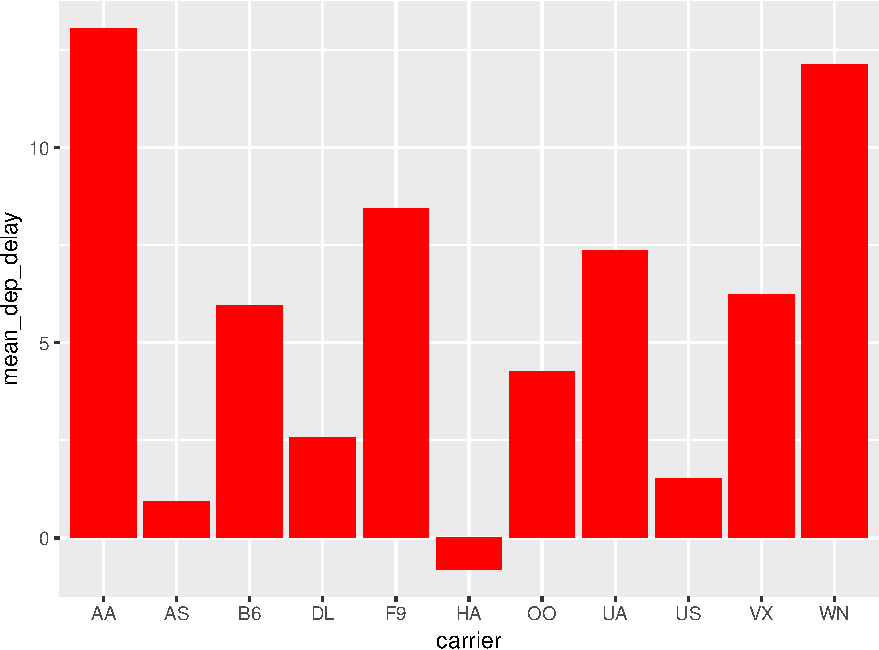
\includegraphics{thesis_files/figure-latex/delaysboxplot-1.pdf}
\caption{\label{fig:delaysboxplot}Mean Delays by Airline}
\end{figure}
Here is a reference to this image: Figure \ref{fig:delaysboxplot}.

A table linking these carrier codes to airline names is available at
\url{https://github.com/ismayc/pnwflights14/blob/master/data/airlines.csv}.

\clearpage

Next, we will explore the use of the \texttt{out.extra} chunk option,
which can be used to shrink or expand an image loaded from a file by
specifying \texttt{"scale=\ "}. Here we use the mathematical graph
stored in the ``subdivision.pdf'' file.
\begin{figure}
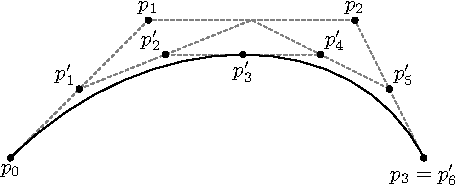
\includegraphics[scale=0.75]{figure/subdivision} \caption{Subdiv. graph}\label{fig:subd}
\end{figure}
Here is a reference to this image: Figure \ref{fig:subd}. Note that
\texttt{echo=FALSE} is specified so that the \textbf{R} code is hidden
in the document.

\textbf{More Figure Stuff}

Lastly, we will explore how to rotate and enlarge figures using the
\texttt{out.extra} chunk option. (Currently this only works in the PDF
version of the book.)
\begin{figure}
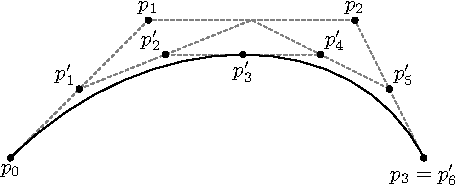
\includegraphics[angle=180, scale=1.1]{figure/subdivision} \caption{A Larger Figure, Flipped Upside Down}\label{fig:subd2}
\end{figure}
As another example, here is a reference: Figure \ref{fig:subd2}.

\section{Footnotes and Endnotes}\label{footnotes-and-endnotes}

You might want to footnote something.\footnote{footnote text} The
footnote will be in a smaller font and placed appropriately. Endnotes
work in much the same way. More information can be found about both on
the CUS site or feel free to reach out to
\href{mailto:data@reed.edu}{\nolinkurl{data@reed.edu}}.

\section{Bibliographies}\label{bibliographies}

Of course you will need to cite things, and you will probably accumulate
an armful of sources. There are a variety of tools available for
creating a bibliography database (stored with the .bib extension). In
addition to BibTeX suggested below, you may want to consider using the
free and easy-to-use tool called Zotero. The Reed librarians have
created Zotero documentation at
\url{http://libguides.reed.edu/citation/zotero}. In addition, a tutorial
is available from Middlebury College at
\url{http://sites.middlebury.edu/zoteromiddlebury/}.

\emph{R Markdown} uses \emph{pandoc} (\url{http://pandoc.org/}) to build
its bibliographies. One nice caveat of this is that you won't have to do
a second compile to load in references as standard LaTeX requires. To
cite references in your thesis (after creating your bibliography
database), place the reference name inside square brackets and precede
it by the ``at'' symbol. For example, here's a reference to a book about
worrying: (Molina \& Borkovec, 1994). This \texttt{Molina1994} entry
appears in a file called \texttt{thesis.bib} in the \texttt{bib} folder.
This bibliography database file was created by a program called BibTeX.
You can call this file something else if you like (look at the YAML
header in the main .Rmd file) and, by default, is to placed in the
\texttt{bib} folder.

For more information about BibTeX and bibliographies, see our CUS site
(\url{http://web.reed.edu/cis/help/latex/index.html})\footnote{Reed~College
  (2007)}. There are three pages on this topic: \emph{bibtex} (which
talks about using BibTeX, at
\url{http://web.reed.edu/cis/help/latex/bibtex.html}),
\emph{bibtexstyles} (about how to find and use the bibliography style
that best suits your needs, at
\url{http://web.reed.edu/cis/help/latex/bibtexstyles.html}) and
\emph{bibman} (which covers how to make and maintain a bibliography by
hand, without BibTeX, at
\url{http://web.reed.edu/cis/help/latex/bibman.html}). The last page
will not be useful unless you have only a few sources.

If you look at the YAML header at the top of the main .Rmd file you can
see that we can specify the style of the bibliography by referencing the
appropriate csl file. You can download a variety of different style
files at \url{https://www.zotero.org/styles}. Make sure to download the
file into the csl folder.

\textbf{Tips for Bibliographies}
\begin{itemize}
\tightlist
\item
  Like with thesis formatting, the sooner you start compiling your
  bibliography for something as large as thesis, the better. Typing in
  source after source is mind-numbing enough; do you really want to do
  it for hours on end in late April? Think of it as procrastination.
\item
  The cite key (a citation's label) needs to be unique from the other
  entries.
\item
  When you have more than one author or editor, you need to separate
  each author's name by the word ``and'' e.g.
  \texttt{Author\ =\ \{Noble,\ Sam\ and\ Youngberg,\ Jessica\},}.
\item
  Bibliographies made using BibTeX (whether manually or using a manager)
  accept LaTeX markup, so you can italicize and add symbols as
  necessary.
\item
  To force capitalization in an article title or where all lowercase is
  generally used, bracket the capital letter in curly braces.
\item
  You can add a Reed Thesis citation\footnote{Noble (2002)} option. The
  best way to do this is to use the phdthesis type of citation, and use
  the optional ``type'' field to enter ``Reed thesis'' or
  ``Undergraduate thesis.''
\end{itemize}
\section{Anything else?}\label{anything-else}

If you'd like to see examples of other things in this template, please
contact the Data @ Reed team (email
\href{mailto:data@reed.edu}{\nolinkurl{data@reed.edu}}) with your
suggestions. We love to see people using \emph{R Markdown} for their
theses, and are happy to help.

\chapter*{Conclusion}\label{conclusion}
\addcontentsline{toc}{chapter}{Conclusion}

If we don't want Conclusion to have a chapter number next to it, we can
add the \texttt{\{-\}} attribute.

\textbf{More info}

And here's some other random info: the first paragraph after a chapter
title or section head \emph{shouldn't be} indented, because indents are
to tell the reader that you're starting a new paragraph. Since that's
obvious after a chapter or section title, proper typesetting doesn't add
an indent there.

\appendix

\chapter{The First Appendix}\label{the-first-appendix}

This first appendix includes all of the R chunks of code that were
hidden throughout the document (using the \texttt{include\ =\ FALSE}
chunk tag) to help with readibility and/or setup.

\textbf{In the main Rmd file}
\begin{Shaded}
\begin{Highlighting}[]
\CommentTok{# This chunk ensures that the thesisdown package is}
\CommentTok{# installed and loaded. This thesisdown package includes}
\CommentTok{# the template files for the thesis.}
\ControlFlowTok{if}\NormalTok{(}\OperatorTok{!}\KeywordTok{require}\NormalTok{(devtools))}
  \KeywordTok{install.packages}\NormalTok{(}\StringTok{"devtools"}\NormalTok{, }\DataTypeTok{repos =} \StringTok{"http://cran.rstudio.com"}\NormalTok{)}
\ControlFlowTok{if}\NormalTok{(}\OperatorTok{!}\KeywordTok{require}\NormalTok{(thesisdown))}
\NormalTok{  devtools}\OperatorTok{::}\KeywordTok{install_github}\NormalTok{(}\StringTok{"ismayc/thesisdown"}\NormalTok{)}
\KeywordTok{library}\NormalTok{(thesisdown)}
\end{Highlighting}
\end{Shaded}
\textbf{In Chapter \ref{ref-labels}:}
\begin{Shaded}
\begin{Highlighting}[]
\CommentTok{# This chunk ensures that the thesisdown package is}
\CommentTok{# installed and loaded. This thesisdown package includes}
\CommentTok{# the template files for the thesis and also two functions}
\CommentTok{# used for labeling and referencing}
\ControlFlowTok{if}\NormalTok{(}\OperatorTok{!}\KeywordTok{require}\NormalTok{(devtools))}
  \KeywordTok{install.packages}\NormalTok{(}\StringTok{"devtools"}\NormalTok{, }\DataTypeTok{repos =} \StringTok{"http://cran.rstudio.com"}\NormalTok{)}
\ControlFlowTok{if}\NormalTok{(}\OperatorTok{!}\KeywordTok{require}\NormalTok{(dplyr))}
    \KeywordTok{install.packages}\NormalTok{(}\StringTok{"dplyr"}\NormalTok{, }\DataTypeTok{repos =} \StringTok{"http://cran.rstudio.com"}\NormalTok{)}
\ControlFlowTok{if}\NormalTok{(}\OperatorTok{!}\KeywordTok{require}\NormalTok{(ggplot2))}
    \KeywordTok{install.packages}\NormalTok{(}\StringTok{"ggplot2"}\NormalTok{, }\DataTypeTok{repos =} \StringTok{"http://cran.rstudio.com"}\NormalTok{)}
\ControlFlowTok{if}\NormalTok{(}\OperatorTok{!}\KeywordTok{require}\NormalTok{(ggplot2))}
    \KeywordTok{install.packages}\NormalTok{(}\StringTok{"bookdown"}\NormalTok{, }\DataTypeTok{repos =} \StringTok{"http://cran.rstudio.com"}\NormalTok{)}
\ControlFlowTok{if}\NormalTok{(}\OperatorTok{!}\KeywordTok{require}\NormalTok{(thesisdown))\{}
  \KeywordTok{library}\NormalTok{(devtools)}
\NormalTok{  devtools}\OperatorTok{::}\KeywordTok{install_github}\NormalTok{(}\StringTok{"ismayc/thesisdown"}\NormalTok{)}
\NormalTok{  \}}
\KeywordTok{library}\NormalTok{(thesisdown)}
\NormalTok{flights <-}\StringTok{ }\KeywordTok{read.csv}\NormalTok{(}\StringTok{"data/flights.csv"}\NormalTok{)}
\end{Highlighting}
\end{Shaded}
\chapter{The Second Appendix, for
Fun}\label{the-second-appendix-for-fun}

\backmatter

\chapter*{References}\label{references}
\addcontentsline{toc}{chapter}{References}

\markboth{References}{References}

\noindent

\setlength{\parindent}{-0.20in} \setlength{\leftskip}{0.20in}
\setlength{\parskip}{8pt}

\hypertarget{refs}{}
\hypertarget{ref-angel2000}{}
Angel, E. (2000). \emph{Interactive computer graphics : A top-down
approach with opengl}. Boston, MA: Addison Wesley Longman.

\hypertarget{ref-angel2001}{}
Angel, E. (2001a). \emph{Batch-file computer graphics : A bottom-up
approach with quicktime}. Boston, MA: Wesley Addison Longman.

\hypertarget{ref-angel2002a}{}
Angel, E. (2001b). \emph{Test second book by angel}. Boston, MA: Wesley
Addison Longman.

\hypertarget{ref-Molina1994}{}
Molina, S. T., \& Borkovec, T. D. (1994). The Penn State worry
questionnaire: Psychometric properties and associated characteristics.
In G. C. L. Davey \& F. Tallis (Eds.), \emph{Worrying: Perspectives on
theory, assessment and treatment} (pp. 265--283). New York: Wiley.

\hypertarget{ref-noble2002}{}
Noble, S. G. (2002). \emph{Turning images into simple line-art}
(Undergraduate thesis). Reed College.

\hypertarget{ref-reedweb2007}{}
Reed~College. (2007, March). LaTeX your document. Retrieved from
\url{http://web.reed.edu/cis/help/LaTeX/index.html}


% Index?

\end{document}
